\section{Implementation}
Before explaining how the modifications for SA-rough were implemented, a couple
of words about the architecture of ADflow are needed.

\paragraph{Block architecture}
This solver only reads \textit{structured grids}, this means all state and grid
variables can be represented in a ``three dimensional table''. One can also think
of a 3d array. This organization is called the \textit{block architecture}. The
index of the block variables are \texttt{i}, \texttt{j} and \texttt{k} for the
x, y and z directions respectively.

\paragraph{Boundary Conditions}
ADflow saves the values of the boundary conditions in a similar way as the block
variables. But they are 2d arrays where the indexes \texttt{i} and \texttt{j}
are used. It is possible to directly relate a volume cell in the block to a
surface cell at the boundary, but it is important to realise surface and volume
cells are different entities.

\paragraph{Global Cell ID}
ADflow assigns a \textit{global cell id} (\texttt{gID} to each volume cell. The
index is an continuously increasing integer that starts at \textbf{0}. It is
applied in a systematic manner that will not be explained further.

\paragraph{Block splitting}
ADflow is capable of solving the governing equations by parallel means. To make
this possible, the whole mesh is split in different blocks. Each processor then
only loads its corresponding block. It is important to realize that no single
processor has access to the whole volume or surface cells\footnote{Assuming more
than one processor is used}.

\subsection{General thoughts}
This modifications requires a little bit more RAM and cpu power. It could also
obscure the standard implementation of the SA model. To cater those
considerations, an on/off switch has been introduced in the python layer called
\texttt{useRoughSA}. When it is \texttt{False}, all implemented changes are
disabled and ADflow behaves exactly as it did before.


\subsection{Changes to wall distance}
The regular SA model needs the distance to the nearest wall. ADflow computes
this distance in a preprocessing step and saves it as a block variable
\texttt{d2wall} for further use. It is slightly more complicated as ADflow can
handle warping meshes and thus this distance needs to be adjusted after each
warp, but this will be explained in more detail later. As shown in equation
\ref{eq:d_new}, the distance to the nearest wall needs to be modified. There are
two strategies to achieve this:

\begin{enumerate}
  \item Overwrite the current \texttt{d2wall} with the modified value. E.g. do
        the modification in a preprocessing step.
  \item Keep the current \texttt{d2wall} as it is and apply the modification
        later when the distance is actually needed.
\end{enumerate}

\noindent Strategy (2) has been chosen as changing the \texttt{d2wall} might
have unforeseen consequences and is just obscuring. But this means, a new block
variable \texttt{ks} needs to be introduced. It will hold the roughness value of
the nearest surface.

\subsubsection{Calculating the distance to the nearest wall}
To be able to assign the correct roughness value of the nearest wall, one must
know which wall is nearest to the current volume cell. For the calculation of
the wall distance, this information is already needed. Thus it was natural to
adapt this function. To explain the changes, one must know how it works:

\begin{enumerate}
  \item The function \texttt{buildClusterWalls} is called. It figures out which
surface mesh belongs to the \textit{no-slip wall} type and gathers all of it on
each processor. This does not scale. But it is assumed the surface mesh is
orders of magnitudes smaller than the volume mesh.  Thus this only becomes a
problem when the size of the volume mesh approaches hundreds of millions of
cells.

Once it has this information, it builds up the whole surface mesh. This is not
straight forward as it might be an overset\footnote{This is also know as Chimera
patch.} mesh where different meshes are overlapping. Therefore it must decide
which cells to drop and which to keep.

After that, it relates the surface mesh to the volume cells and returns the
\texttt{gID}. At first glance, it might seem weird to return ``volume cells''
when the distance to a surface cell is required. But the grid points of both
types are the same and for the walldistance computation the boundary conditions
do not matter.

  \item Once the \texttt{clusterWalls} are built, the function
\texttt{determineWallAssociation} iterates through all the volume cells on the
current processor and figures out which \texttt{gID} of the
\texttt{clusterWalls} is nearest.

Whit that information, it creates a ``PETSc scatter''\footnote{PETSc stands for
Portable, Extensible Toolkit for Scientific Computation.} object called
\texttt{wallScatter}. This object is (in simplified terms) a two dimensional
list which keeps track of which surface cell is nearest to which volume cell. As
the surface cells have been replaced with volume cells before, this is basically
a mapping of volume cells to volume cells.

After that, the memory for \texttt{clusterWalls} is released.

\item A new block variable \texttt{xSurf} is introduced. It holds all the
surface grid points, which are needed for the wall distance calculation for the
volume cells of the current processor. It is the receiving end of the
\texttt{wallScatter} object.

\item In the End, \texttt{updateWallDistancesQuickly} is called to actually
compute the distance to the nearest wall based on the grid points stored in
\texttt{xSurf}.

\item After the mesh has been warped, only \texttt{updateWallDistancesQuickly}
is called. This means, it is assumed the nearest surface cell does not
change, only its coordinates.
\end{enumerate}

\noindent Please note the outlined steps above are in reality a bit more
complicated and only the broad context is described.


\subsubsection{Assigning the block variable \texttt{ks}}
\label{subsubsec:propagate_ks}
To fill the block variable \texttt{ks} with the roughness value of the nearest
surface, the before described walldistance computation is hijacked as follows:

\begin{enumerate}[label=\Alph*]
  \item Introduce a new block variable called \texttt{nearestWallCellInd}. It
holds the \texttt{gID} of the nearest surface cell. Its value is assigned in
step (2) where the \texttt{gID} of the nearest surface cell is determined.

  \item Create a new subroutine called \texttt{updateWallRoughness}. A separate
subroutine is needed as the roughness value on the boundary is only read from
the CGNS\footnote{CGNS stands for CFD General Notation System and is a format
for meshes and their solutions. It is the primary format that ADflow interacts
with.} file once the walldistance has already been calculated. Thus it is not
possible to do it when step (2) is done. ADflow has some helper functions that
allows to overwrite the values of the boundary conditions which are saved in the
CGNS file. Having a separate subroutine to assign \texttt{ks} allows to also use
those helper functions for the wall roughness.
\end{enumerate}

\noindent Now, the inner workings of \texttt{updateWallRoughness} are explained
in more detail:

\begin{enumerate}[label=\Alph*]
  \item Each processor creates two lists: (a) the roughness values of the
surface cells on current processor and (b) the corresponding \texttt{gID}.

  \item Then those two lists are gathered on all processors. This means, every
processor has a list ($\alpha$) of all surface roughness values and ($\beta$) of
all corresponding \texttt{gID}. This does also not scale. But this constraint
has been violated before (in \texttt{buildClusterWalls}) and thus the totally
required RAM is not increased significantly.

\item Now, each processor iterates through its volume cells and requests the
\texttt{gID} from \texttt{nearestWallCellInd}. Then it searches list ($\beta$)
until it finds the same \texttt{gID} and writes down the index \texttt{I} where
it found it.

\item Finally, it assigns the value of list ($\alpha$) at index \texttt{I} to the
block variable \texttt{ks}.
\end{enumerate}

\noindent It is important to note that this strategy can handle different
roughness values for the surface. But those values are not interpolated and are
thus only accurate in the limiting sense of an infinitely fine grid. It can also
lead to weird situations where one single volume cell is assigned a roughness
value where as its surrounding cells are not. This happens because its center is
somehow closest to a small corner of a rough surface cell. This also vanishes
with increasing cell count.

\subsection{SA source terms}
As described in section \ref{subsec:mod_sa_rough}, the terms $\chi$ (equation
\ref{eq:chi_new}) and $f_{v2}$ (equation \ref{eq:fv2_new}) need to be modified.
This has been straight forward. But it is important to not forget the
calculation of $d_{new}$ (equation \ref{eq:d_new}) as this has been postponed in
the previous section.

ADflow employs some Newton-type solvers that require the Jacobian of the
resiudals. Thus it was necessary to also modify the derivative of
$\partial f_{v2} / \partial \tilde \nu$ as follows:

\begin{equation}
  \frac{\partial f_{v2}}{\partial \tilde \nu} =
  \frac{\tilde \nu^{2} \frac{\partial f_{v1}}{\partial \tilde \nu} - \nu}
  {(\tilde \nu f_{v1} + \nu)^{2}}
\end{equation}

\noindent As said before, those changes are only active when \texttt{useRoughSA}
is \texttt{True}.

\subsection{SA boundary conditions}
ADflow employs the concept of \textit{halo cells}. This is an idea to exchange
the boundaries of the split blocks when running in parallel. Take a look at
figure \ref{fig:halo_cells}. On the left side, a block split in 4 is shown. Each
sub-block lives on a different processor. On the right, one can see the
artificial halo cells. After each iteration of the flow solver, the values of
the halo cells are updated with their corresponding values of the other blocks
(red arrows).

\begin{figure}[H] \centering
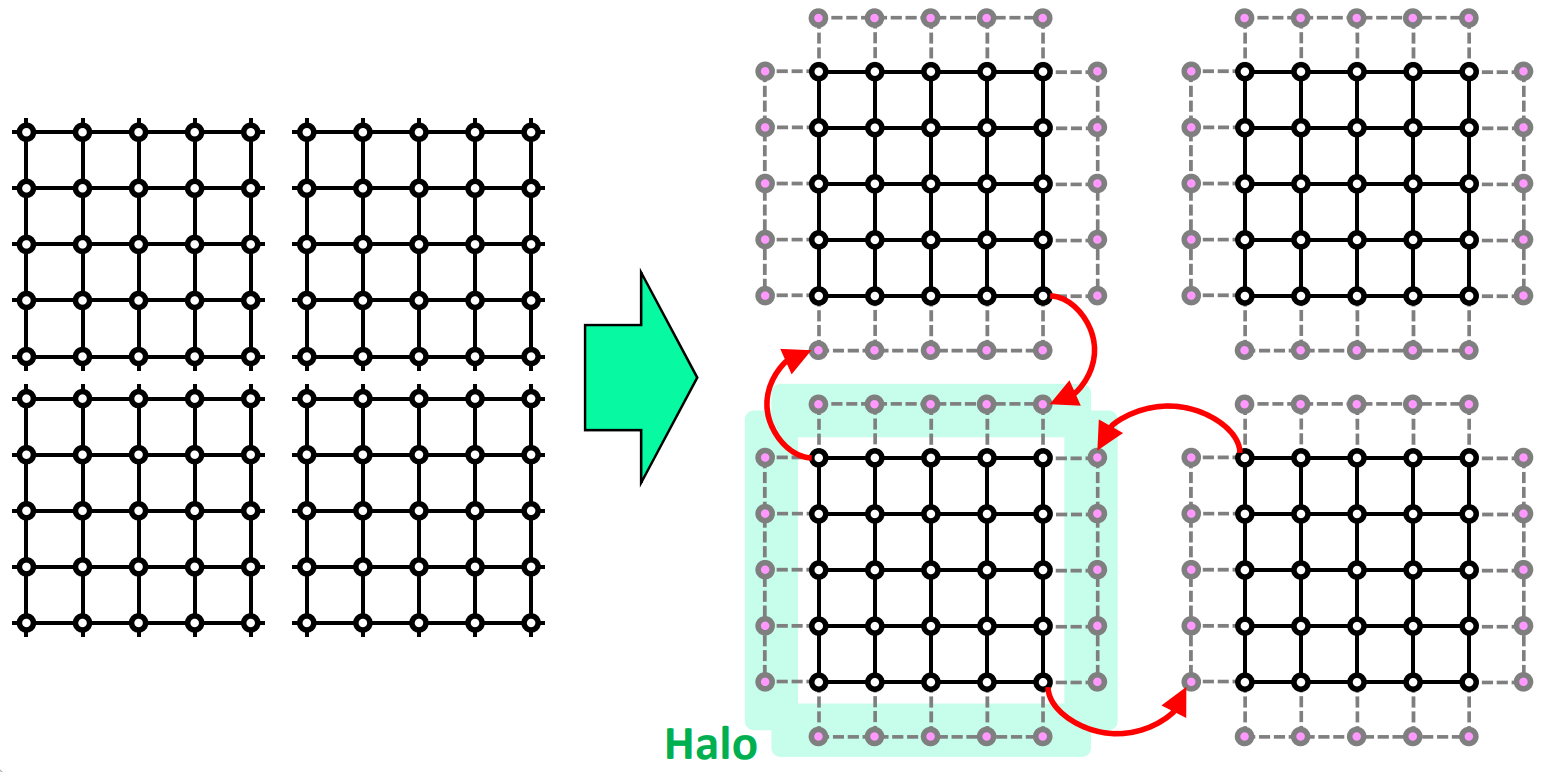
\includegraphics[width=0.7\textwidth]{halo_cells}
    \caption{A block split in 4 (left) and its corresponding halo cells (right)
            \cite{cfd_halo}.}
    \label{fig:halo_cells}
\end{figure}

ADflow is capable of deploying second order schemes and thus needs two layers of
halo cells. But the idea remains the same. As they are not always active, ADflow
takes care of interpolating them by itself.

\paragraph{Explicit boundary conditions}
The concept of halo cells can also be used to prescribe the regular boundary
conditions like a \textit{no-slip wall}. According to equation
\ref{eq:sa_nu_wall_0}, the regular SA model needs a boundary condition of
$\tilde \nu_{wall} = 0$. This means, the first halo is simply updated with the
negative value of the first cell:

\begin{equation}
  \tilde \nu_{h} = - \tilde \nu_{1} \qquad \rightarrow \qquad
  \tilde \nu_{wall} = \frac{\tilde \nu_{1} + \tilde \nu_{h}}{2} = 0
  \label{eq:bc_halo}
\end{equation}

\noindent Where $\tilde \nu_{1}$ is the value of the first interior cell and
$\tilde \nu_{h}$ is the halo cell.

For the rough version, the boundary condition needs to be modified according to
equation \ref{eq:bc_new}:

\begin{equation}
  \left( \frac{\partial \tilde \nu}{\partial n} \right) \equiv
  \frac{\tilde \nu_{1} - \tilde \nu_{h}}{d} =
  \frac{\tilde \nu_{wall}}{0.03 k_{s}}
\end{equation}

\noindent Replacing $\tilde \nu_{wall}$ with equation \ref{eq:bc_halo} and
solving for $\tilde \nu_{h}$, one gets:

\begin{equation}
  \tilde \nu_{h} = \tilde \nu_{1} \frac{0.06 k_{s} - d}{0.06 k_{s} + d}
\end{equation}

\noindent The underlying assumption is, that the first cell to the wall is not
skewed and its center is normal to the wall. But this is in general good practice
and highly recommended for RANS meshes.


\paragraph{Implicit boundary conditions}
ADflow also has some implicit solvers, thus the implicit boundary conditions need to be changed.

TBD!!!!

\subsection{Automatic Differentiation}
As described in \cite{cm1}, ADflow uses Automatic/Algorithmic Differentiation to
compute the partial derivatives which are needed in the \textit{adjoint method}
to compute the total derivatives of the functions of interest with respect to
the design variables. The AD tool used is called \textit{tapenade}
\cite{tapenade}. It is based on JAVA and directly differentiates Fortran source
code. One provides the source code of a Fortran routine, defines the dependent
output variable and the independent input variable with respect to which the
derivative is requested. Tapenade then returns Fortran source code that
computes this derivative.

When the AD architecture for ADflow was set up, tapenade could not handle
parallelization calls using the MPI\footnote{MPI stands for Message Passing
Interface and handles the communication across different processors and
computers when performing parallel computations.}. Thus the decision was made to
split the whole AD in two parts: part (1) communicates data across different
processors, i.e takes care of the parallelization; and part (2) does the actual
computation. This allows tapenade to differentiate the math heavy part (2) and
necessitates the developer to make sure the differentiated routines are called
appropriately (1).


\section{Verification}
The verification of the SA changes is split into two parts: making sure the
roughness values are propagated correctly into the volume cells and verifying SA
rough does actually behave like a rough wall.

\subsection{Roughness propagation}
\label{subsec:roughness_prop}
When assigning a roughness value to the surface, this value gets propagated to
the volume cells as described in section \ref{subsubsec:propagate_ks}. This has
to be tested, especially when running on multiple processors. To get a chance to
do this, ADflow has been modified to write the \texttt{ks} values to the
solution grid (if requested).

\paragraph{Cube}
The first test is a cube where each face is split into 9 parts. The center of
each face has been prescribed a roughness value of $k_{s} = 1.0$. The rest of
each face gets a value of $k_{s} = 0.1$. Figure \ref{fig:cube_oid_ks_prop} shows
the surface and the corresponding roughness values. This test exists as it easily
verifiable that the propagation looks right.

\paragraph{Cuboid}
The main thing that could fail in this test is the correlation from the surface
cell to the \texttt{gID} as described in section \ref{subsubsec:propagate_ks}.
It is not possible to test this properly when the test case is symmetric. This
necessitated the introduction of a cuboid where a random cell on the surface is
made rough. This can be seen in figure \ref{fig:cube_oid_ks_prop}. The
underlying assumption is that the search for the surface \texttt{gID} fails when
the correlation is wrong. This has been observed in practice.

All volume meshes in this report were generated using pyHyp \cite{Secco2021}. It
reads a surface mesh and extrudes it into the third dimension. But it allways
orients the internal block coordinates (\texttt{i}, \texttt{j} and \texttt{k})
in the same direction such that the \texttt{kMin} face is allways the wall. The
correlation of the surface cell to the \texttt{gID} is different for each block
face. Thus this is a test with 6 different meshes where each block is rotated
such that each face is the wall once.


\begin{figure}[H] \centering
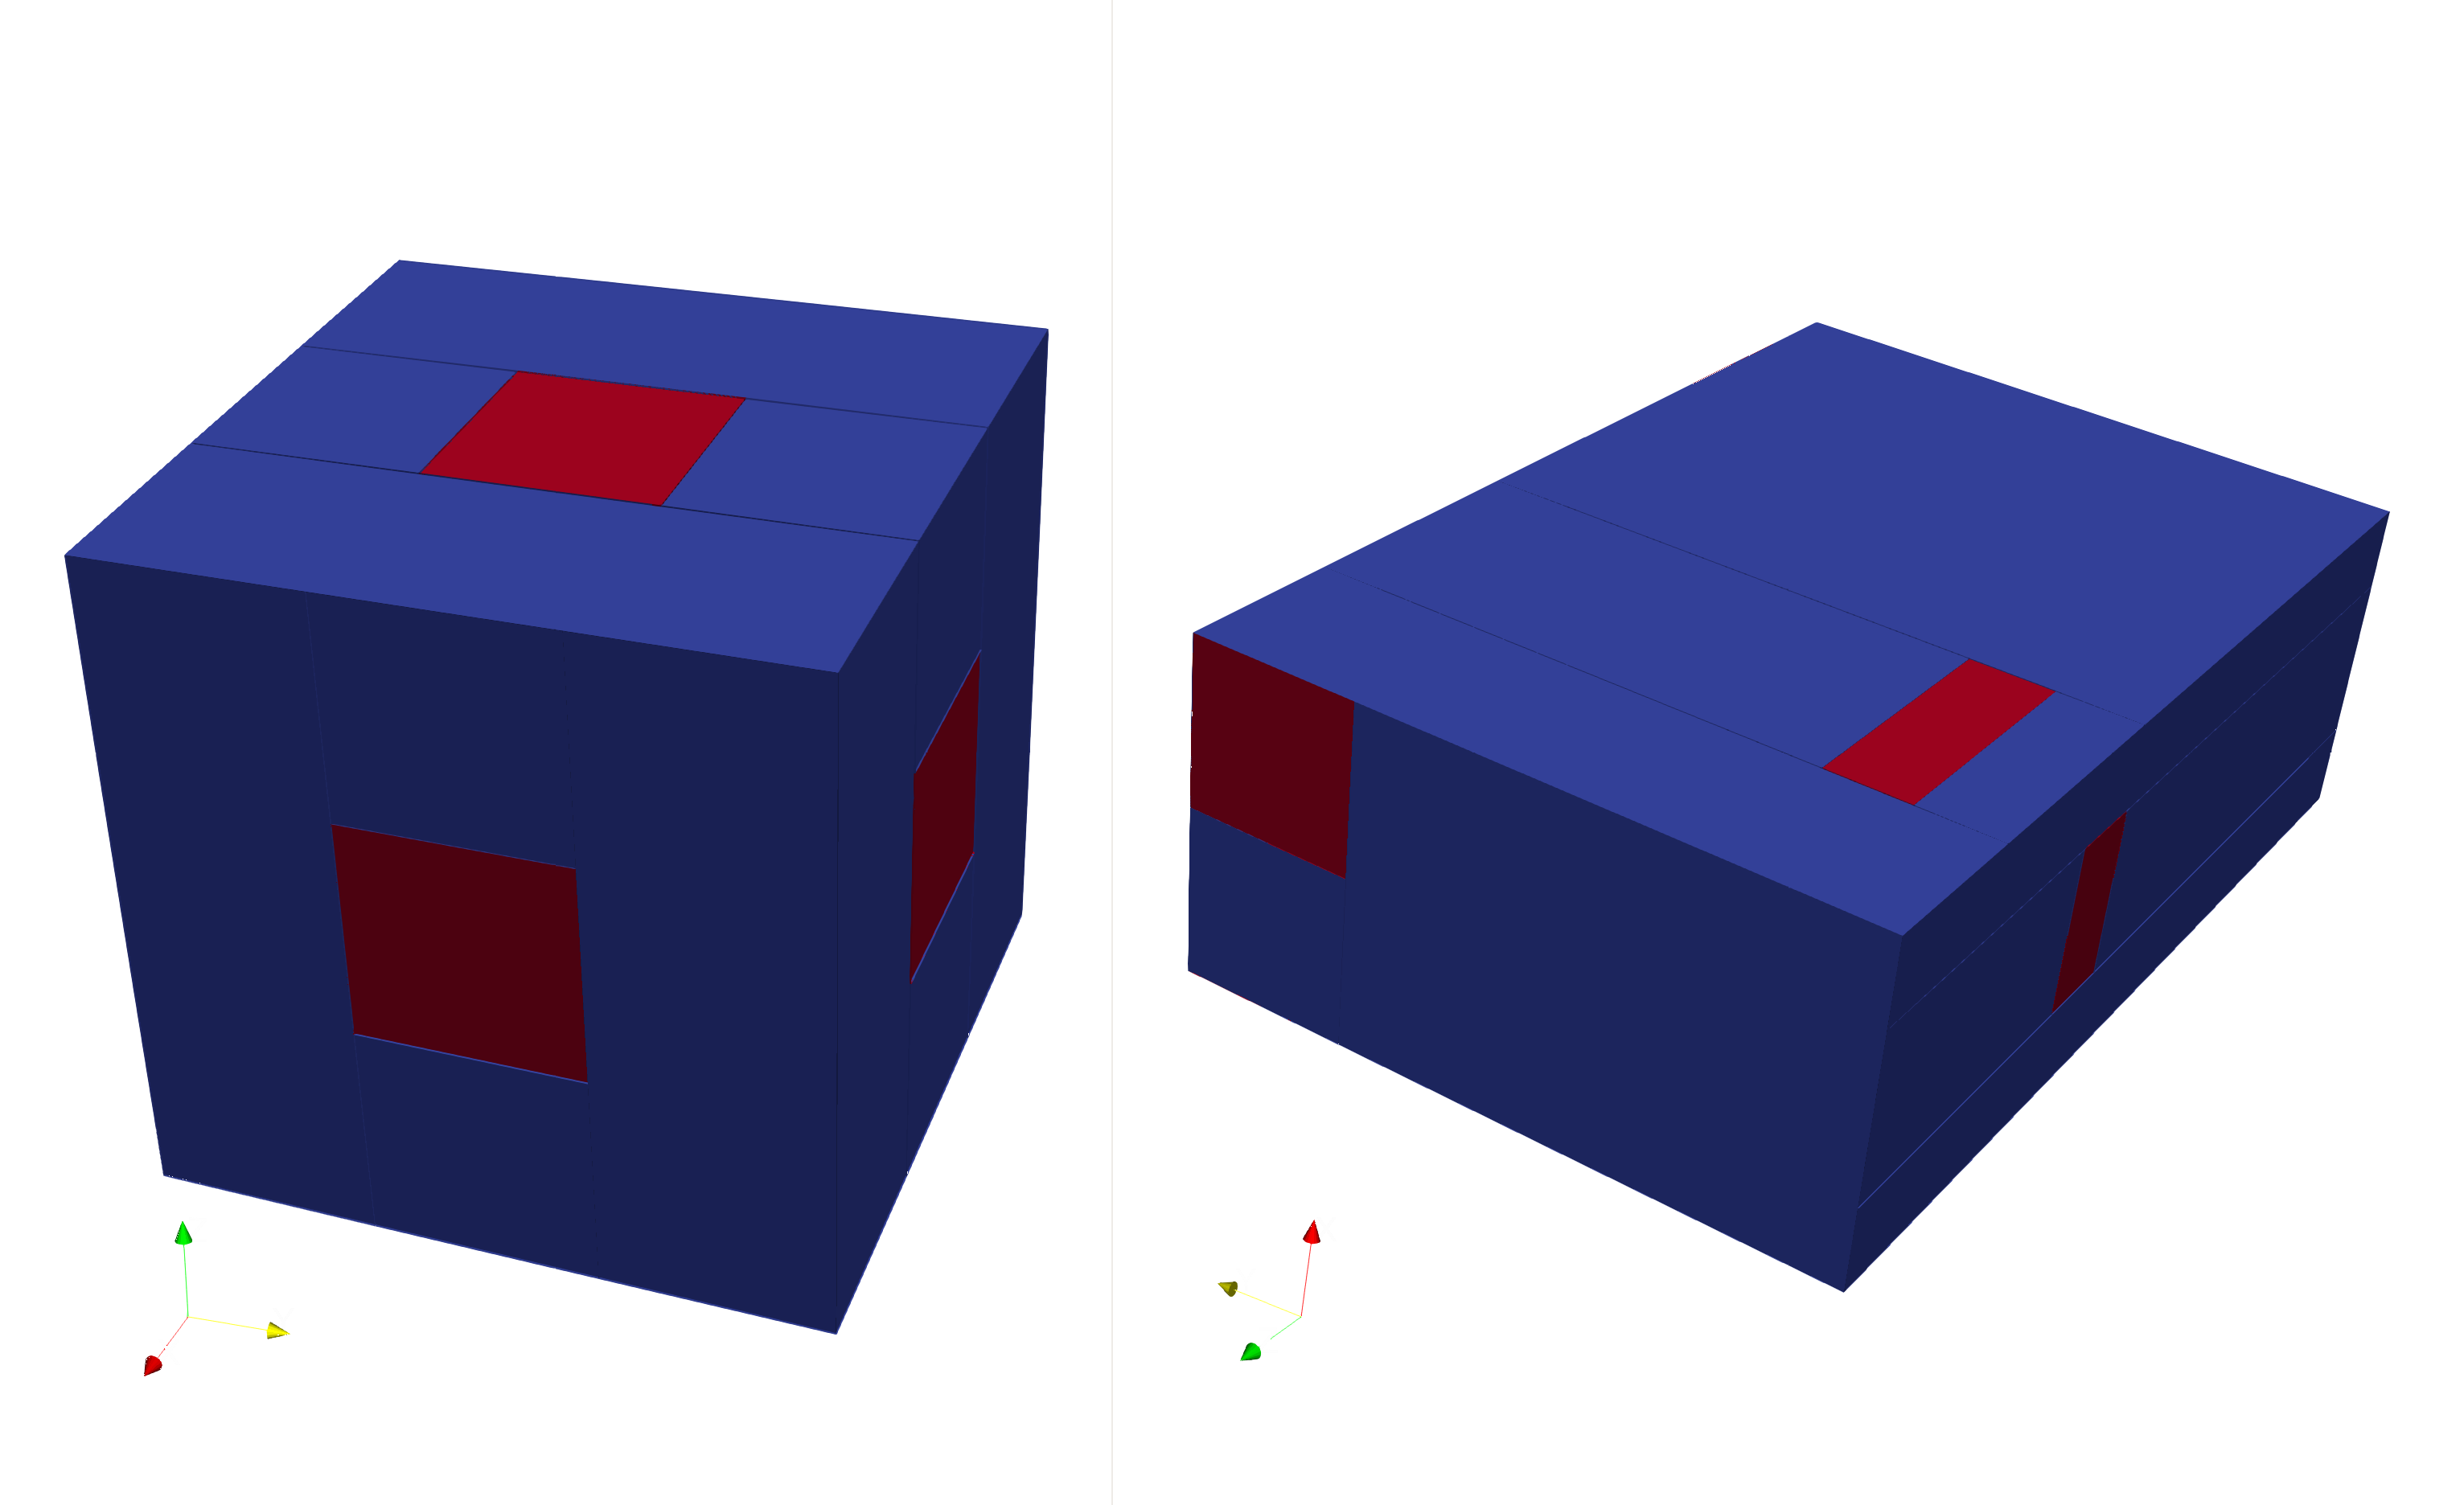
\includegraphics[width=0.7\textwidth]{cube_oid_ks_prop}
    \caption{Cube and cuboid for $k_{s}$ propagation test. Blue means
$k_{s} = 0.1$ and red equals $k_{s} =1.0$.}
    \label{fig:cube_oid_ks_prop}
\end{figure}

\paragraph{Overset cube}
The highjacked subroutine for the wall distance calculation takes a slightly
different path when overset meshes are used. To test it, the cube mesh from
before was repurposed. It was extendend with a coarse Cartesian  background
grid.  ADflow uses the \textit{implicit hole cutting scheme} to decide by itself
how to interpolate between those grids. As this was failing with the initial
grid, it has been refined slightly.

\subsection{Grid Convergence}

TBD

\subsection{Comparisons}
It is necessary to compare the SA rough implementation against theory and
experiments. As it is hard to get experimental data, the \textit{flat plat a
zero incidence} test case has been chosen for all comparisons. NASA maintains a
website called \textit{turbulence modeling resource} \cite{rumsey_flat}. There,
various formulations for different turbulence models may be found. Additionally
it provides testcases, grids and validation data. The following grid-family with
its corresponding boundary conditions was sourced from there (figure
\ref{fig:plate_bc}). Table \ref{tab:plate_sizes} lists the different mesh sizes.

\begin{figure}[H] \centering
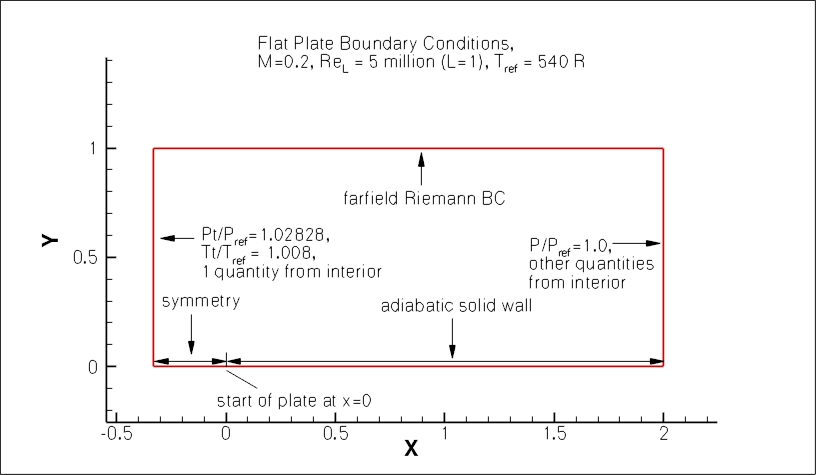
\includegraphics[width=0.7\textwidth]{plate_bc}
    \caption{Boundary conditions and test case overview \cite{rumsey_flat}.}
    \label{fig:plate_bc}
\end{figure}

\begin{table}[H]
  \centering
  \begin{tabular}{c r r}
    Identifier      & \# of nodes   & \# of cells \\
    \toprule
    L4              & 1'800         & 816 \\
    L3              & 6'860         & 3'264 \\
    L2              & 26'772        & 13'056 \\
    L1              & 105'764       & 52'224 \\
    L0              & 420'420       & 208'896 \\

  \end{tabular}
  \caption{Mesh sizes used for testcases.}
  \label{tab:plate_sizes}
\end{table}

\noindent The following cases were set up.

\paragraph{Clean}
The NASA TMR website \cite{rumsey_flat} provides numercial data on the skin
friction coefficient ($c_{f}$) for a clean wall. The SA rough model with a
surface roughness of $k_{s} = 0$ should match.

\paragraph{SU2}
SU2 is an open source solver \cite{su2} that has allready implemented SA rough.
Therefore it was natural to compare both implementations.

\paragraph{Acharya et al.}
Acharya et al. did some experiments with flows of a flat plates over rough walls.


TBD!!!!

\section{Automated tests}

\subsection{Gradients}
